% Options for packages loaded elsewhere
\PassOptionsToPackage{unicode}{hyperref}
\PassOptionsToPackage{hyphens}{url}
%
\documentclass[
]{article}
\usepackage{amsmath,amssymb}
\usepackage{iftex}
\ifPDFTeX
  \usepackage[T1]{fontenc}
  \usepackage[utf8]{inputenc}
  \usepackage{textcomp} % provide euro and other symbols
\else % if luatex or xetex
  \usepackage{unicode-math} % this also loads fontspec
  \defaultfontfeatures{Scale=MatchLowercase}
  \defaultfontfeatures[\rmfamily]{Ligatures=TeX,Scale=1}
\fi
\usepackage{lmodern}
\ifPDFTeX\else
  % xetex/luatex font selection
\fi
% Use upquote if available, for straight quotes in verbatim environments
\IfFileExists{upquote.sty}{\usepackage{upquote}}{}
\IfFileExists{microtype.sty}{% use microtype if available
  \usepackage[]{microtype}
  \UseMicrotypeSet[protrusion]{basicmath} % disable protrusion for tt fonts
}{}
\makeatletter
\@ifundefined{KOMAClassName}{% if non-KOMA class
  \IfFileExists{parskip.sty}{%
    \usepackage{parskip}
  }{% else
    \setlength{\parindent}{0pt}
    \setlength{\parskip}{6pt plus 2pt minus 1pt}}
}{% if KOMA class
  \KOMAoptions{parskip=half}}
\makeatother
\usepackage{xcolor}
\usepackage[margin=1in]{geometry}
\usepackage{graphicx}
\makeatletter
\def\maxwidth{\ifdim\Gin@nat@width>\linewidth\linewidth\else\Gin@nat@width\fi}
\def\maxheight{\ifdim\Gin@nat@height>\textheight\textheight\else\Gin@nat@height\fi}
\makeatother
% Scale images if necessary, so that they will not overflow the page
% margins by default, and it is still possible to overwrite the defaults
% using explicit options in \includegraphics[width, height, ...]{}
\setkeys{Gin}{width=\maxwidth,height=\maxheight,keepaspectratio}
% Set default figure placement to htbp
\makeatletter
\def\fps@figure{htbp}
\makeatother
\setlength{\emergencystretch}{3em} % prevent overfull lines
\providecommand{\tightlist}{%
  \setlength{\itemsep}{0pt}\setlength{\parskip}{0pt}}
\setcounter{secnumdepth}{-\maxdimen} % remove section numbering
\ifLuaTeX
  \usepackage{selnolig}  % disable illegal ligatures
\fi
\usepackage{bookmark}
\IfFileExists{xurl.sty}{\usepackage{xurl}}{} % add URL line breaks if available
\urlstyle{same}
\hypersetup{
  hidelinks,
  pdfcreator={LaTeX via pandoc}}

\author{}
\date{\vspace{-2.5em}}

\begin{document}

\subsection{Figures}\label{figures}

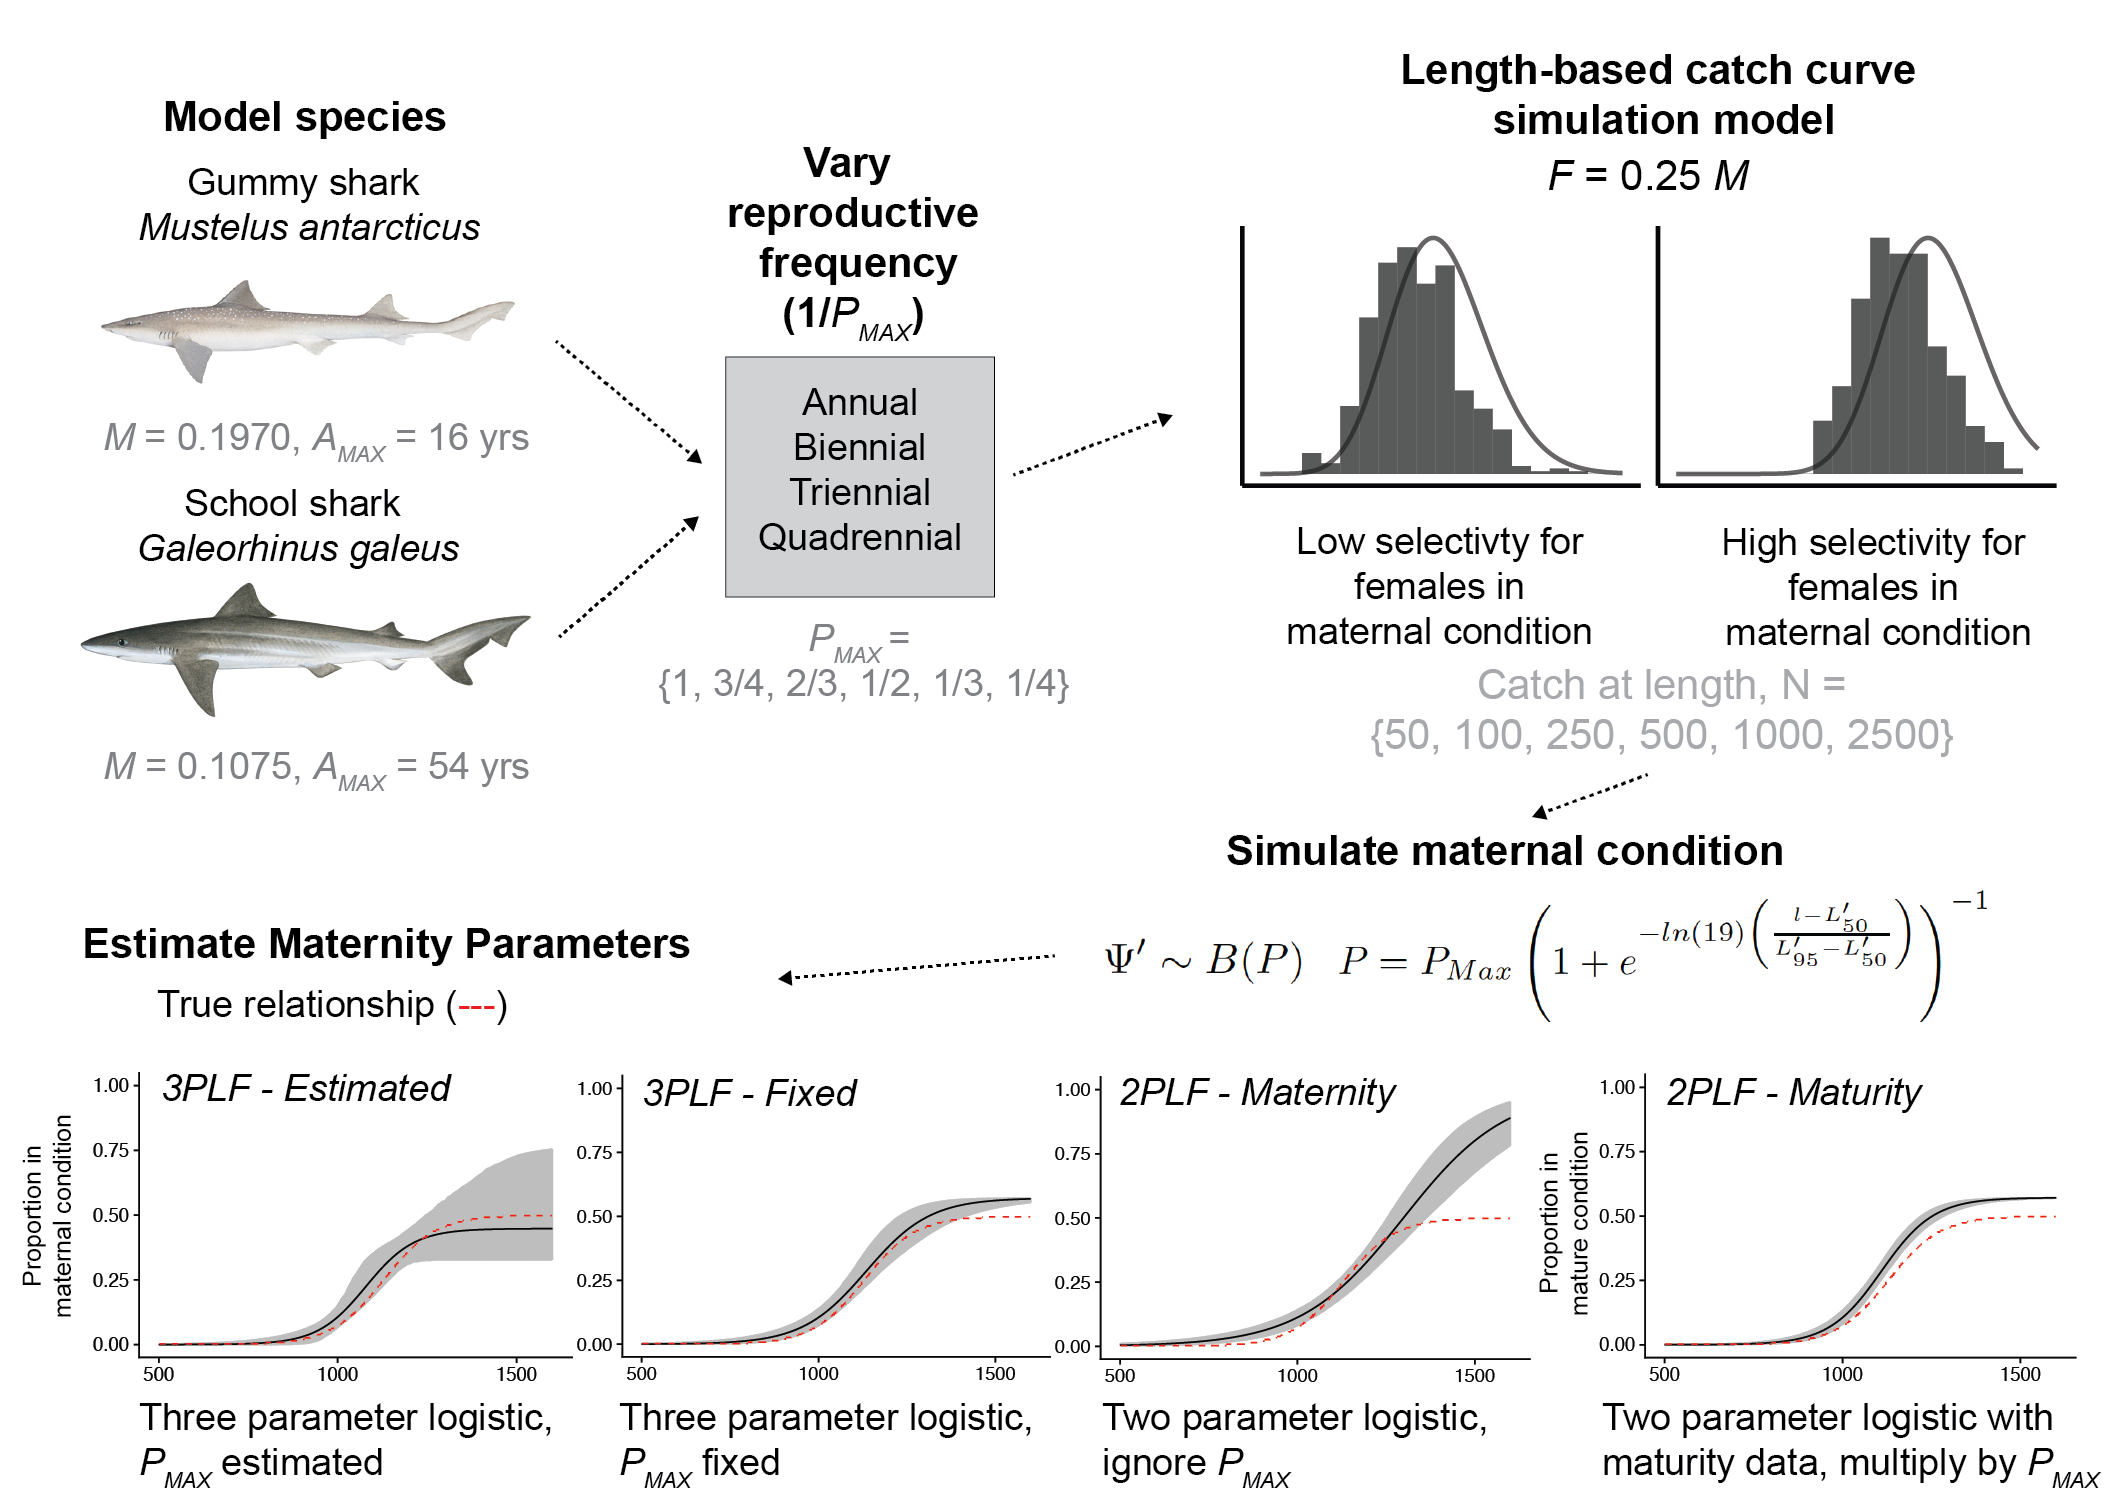
\includegraphics[width=1\linewidth]{../img/figure1}

Figure 1. Approach used to generate simulated data and test the
performance of four methods for calculating maternity parameters.
Illustrations © R.Swainston/www.anima.net.au

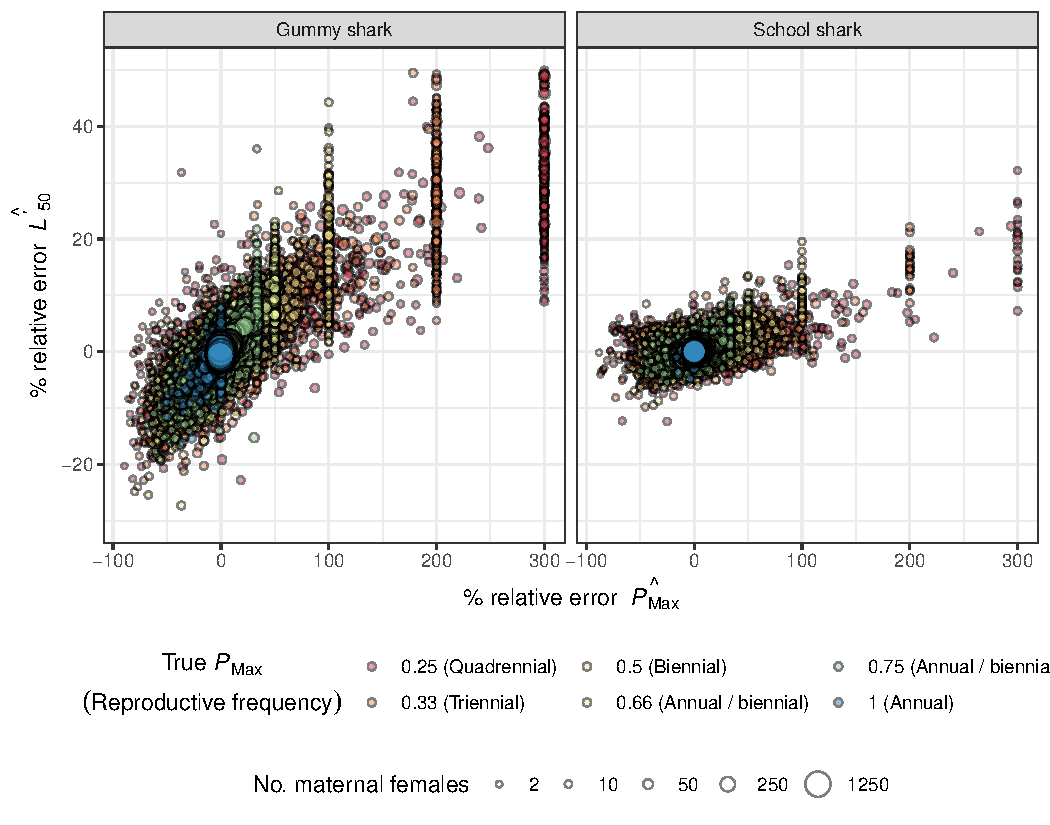
\includegraphics{/Users/avh/Library/CloudStorage/OneDrive-DepartmentofPrimaryIndustriesAndRegionalDevelopment/manuscripts/maternity-function/reports/figs_files/figure-latex/unnamed-chunk-2-1.pdf}

Figure 2. Bias (per cent relative error) in parameter estimates for
\(\hat{L'_{50}}\) and \(\hat{P_{Max}}\) for the 3PLF maternity function
with \(P_{Max}\) estimated. Each point represents parameter estimates
from one iteration of simulated data (n = 43,129), including all
combinations of variables. Simulations with longer reproductive cycles
and fewer maternal females were associated with higher bias in both
\(\hat{L'_{50}}\) and \(\hat{P_{Max}}\). Note: 42 data points were
cropped to aid with data visualization (see Figure S13 for uncropped
figure).\\
\strut \\
\newpage

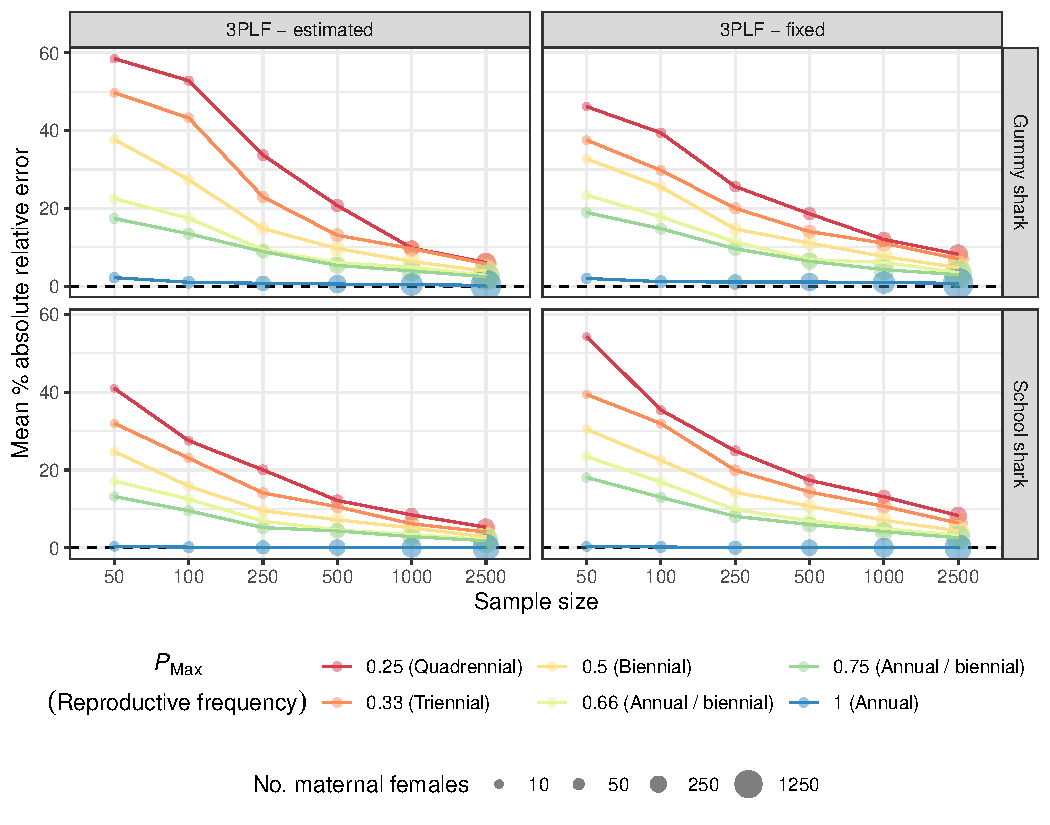
\includegraphics{/Users/avh/Library/CloudStorage/OneDrive-DepartmentofPrimaryIndustriesAndRegionalDevelopment/manuscripts/maternity-function/reports/figs_files/figure-latex/unnamed-chunk-3-1.pdf}

Figure 3. Accuracy (per cent absolute error) in parameter estimates of
\(\hat{P_{Max}}\) for 3PLF methods with high maternal selectivity. Large
sample sizes were needed to accurately estimate \(\hat{P_{Max}}\) and
accuracy decreased as the duration of the reproductive cycle increased.
Each point reflects a mean value from 300 simulated data sets. Point
size denotes mean number of females in maternal condition at a given
sample size.\\
\strut \\
\newpage

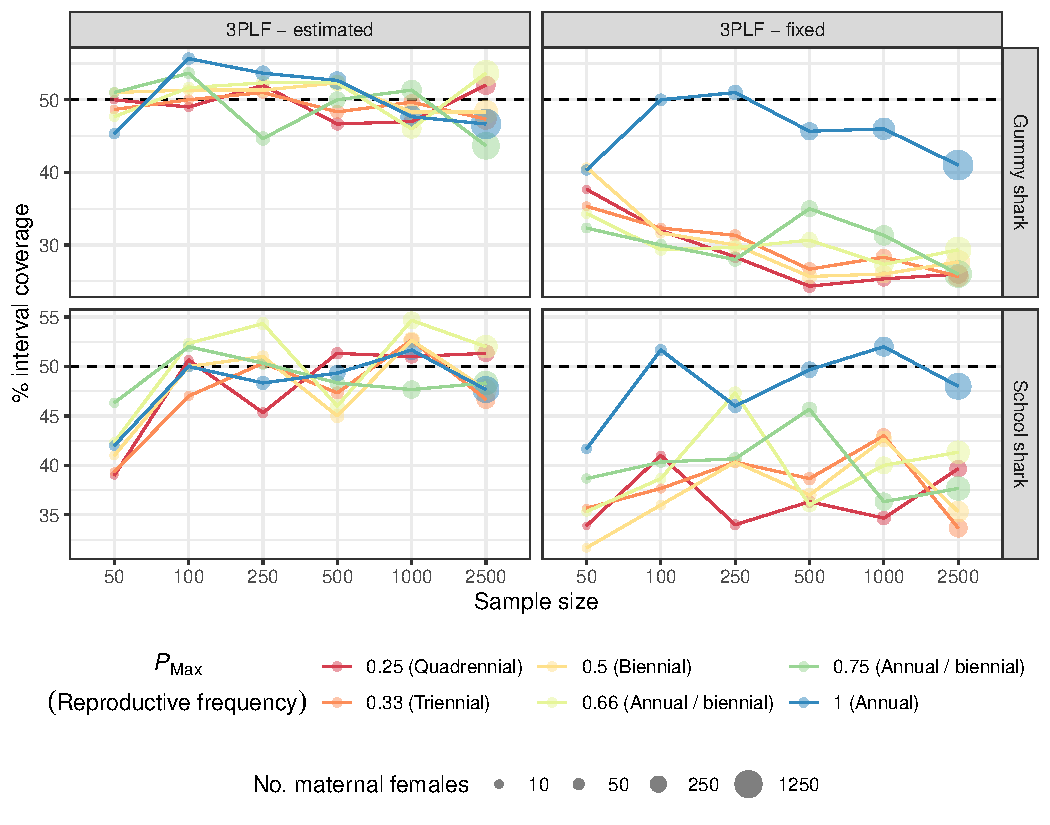
\includegraphics{/Users/avh/Library/CloudStorage/OneDrive-DepartmentofPrimaryIndustriesAndRegionalDevelopment/manuscripts/maternity-function/reports/figs_files/figure-latex/unnamed-chunk-4-1.pdf}

Figure 4. Confidence interval coverage for \(\hat{L'_{50}}\) for 3PLF
methods with high maternal selectivity. Figure shows the percentage of
simulations (n = 300) where the true parameter value fell within the
50\% bootstrap confidence interval. Point size denotes mean number of
females in maternal condition at a given sample size.\\
\strut \\
\newpage

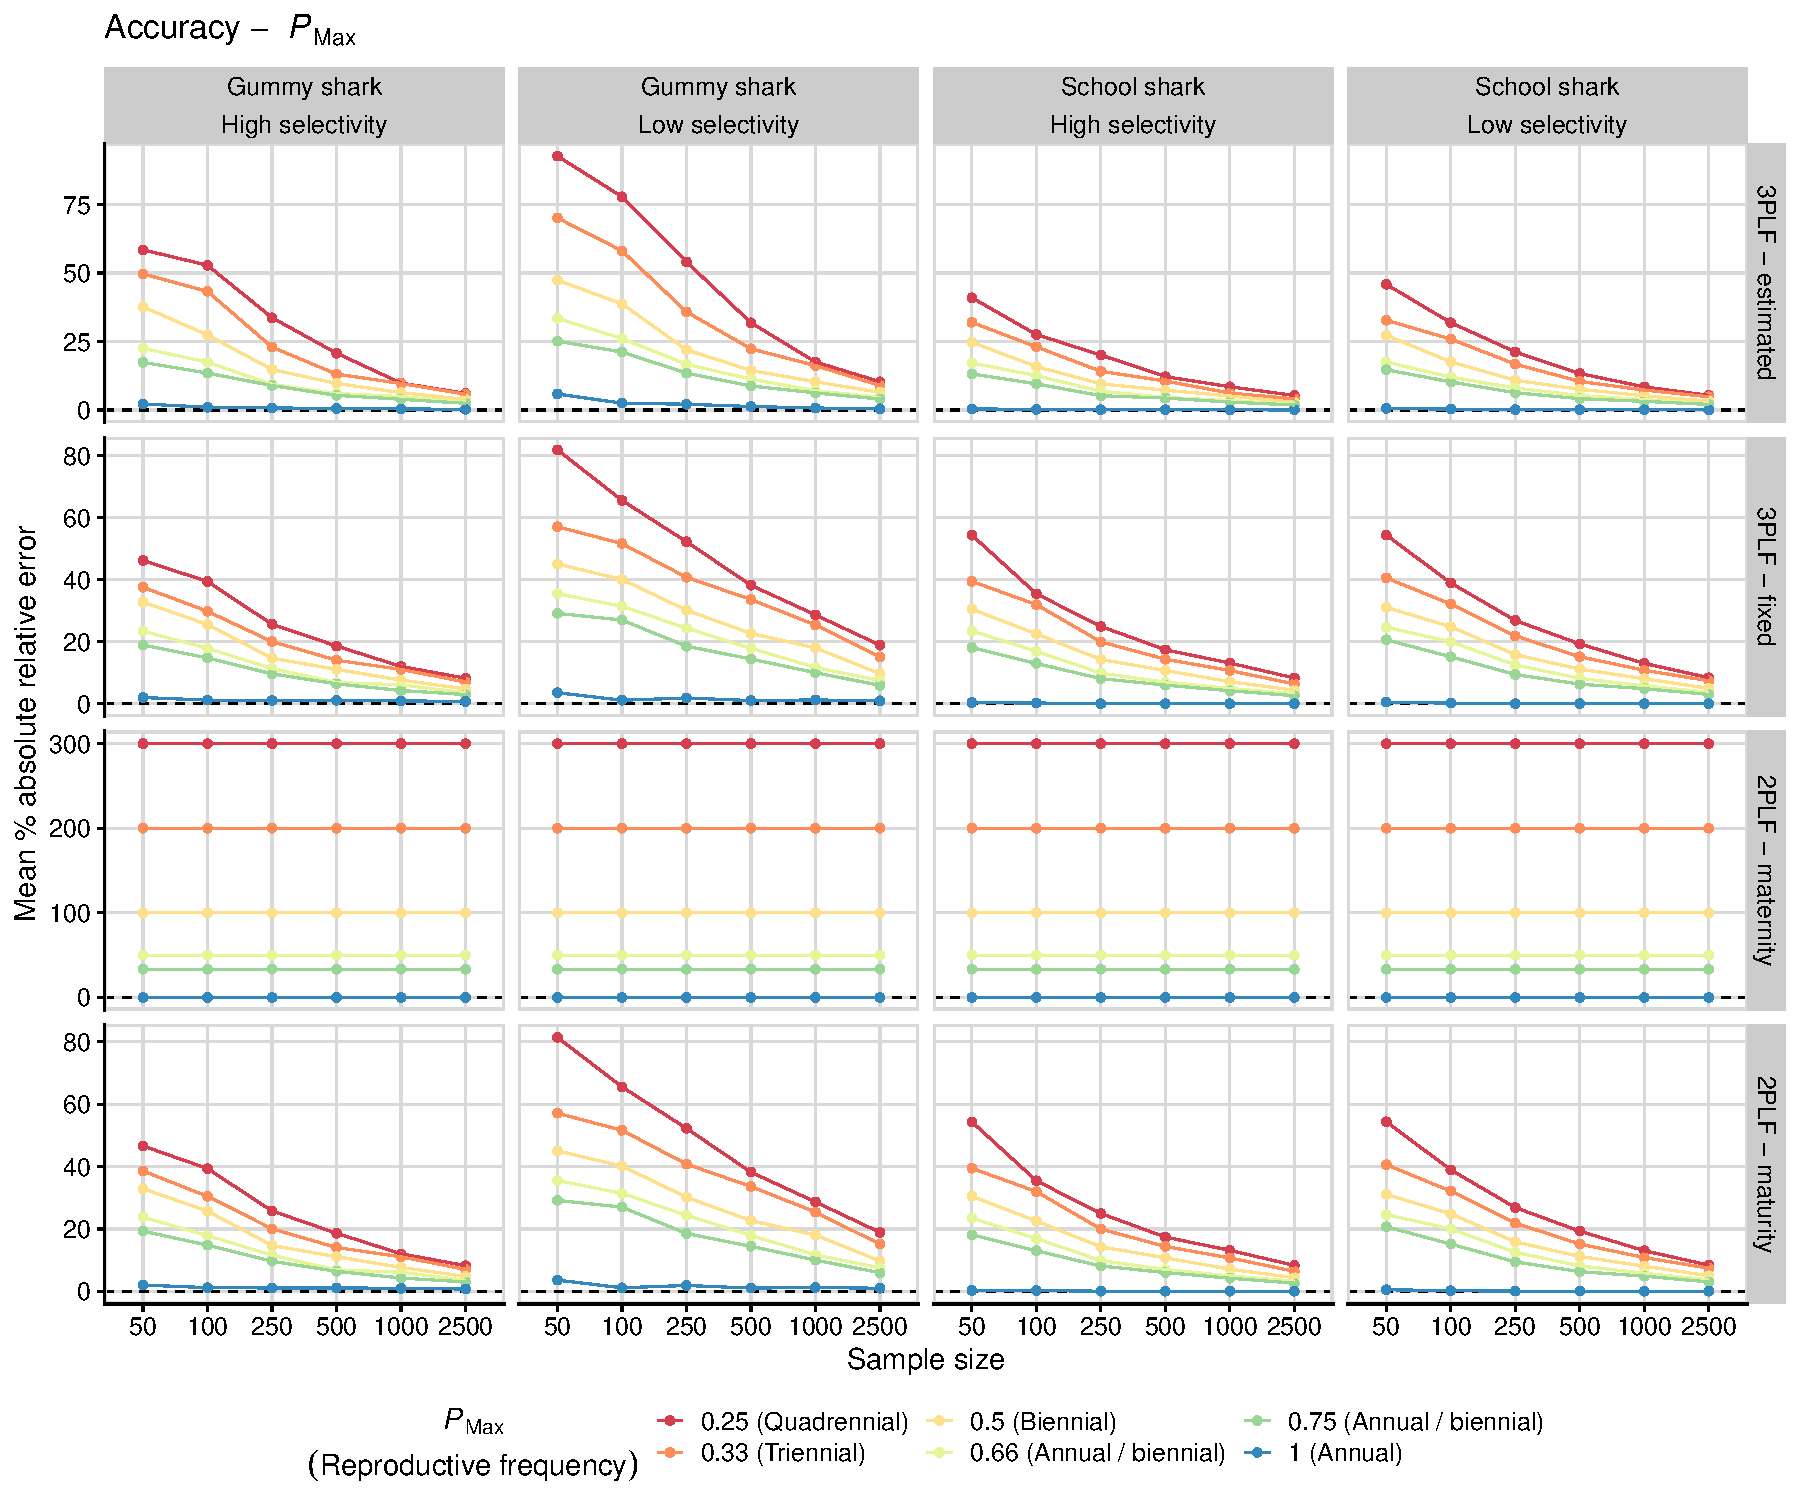
\includegraphics{/Users/avh/Library/CloudStorage/OneDrive-DepartmentofPrimaryIndustriesAndRegionalDevelopment/manuscripts/maternity-function/reports/figs_files/figure-latex/unnamed-chunk-5-1.pdf}

Figure 5. Accuracy (per cent absolute error) in parameter estimates of
\(\hat{P_{Max}}\) for the 3PLF - estimated method as a function of
number of maternal females. Each point reflects a value from 300
simulated data sets.\\
\newpage

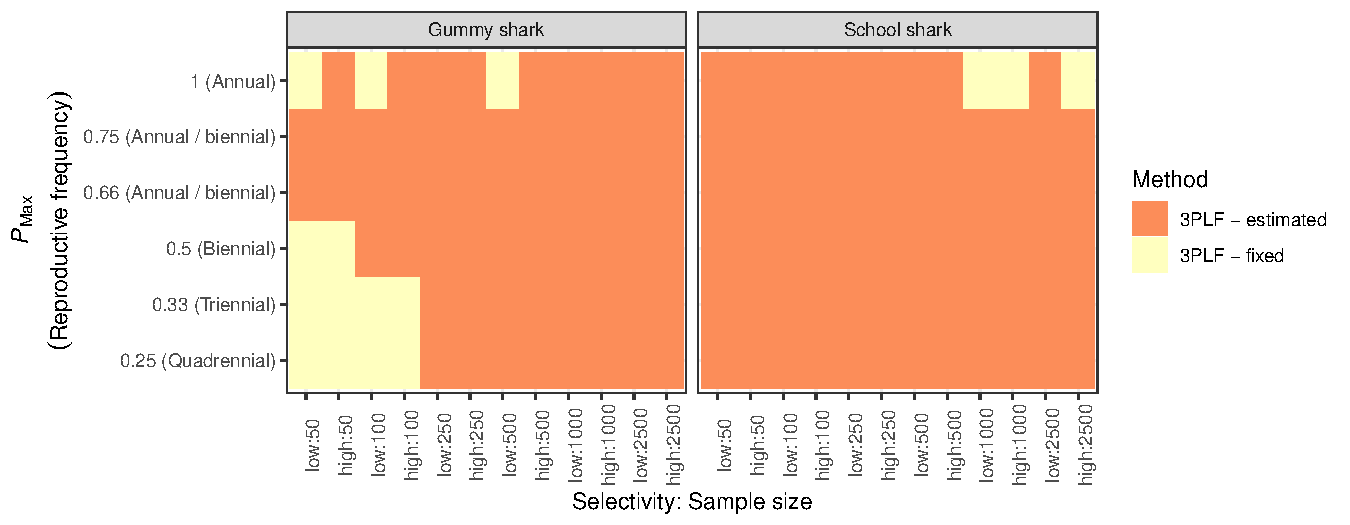
\includegraphics{/Users/avh/Library/CloudStorage/OneDrive-DepartmentofPrimaryIndustriesAndRegionalDevelopment/manuscripts/maternity-function/reports/figs_files/figure-latex/unnamed-chunk-6-1.pdf}

Figure 6. Performance of four alternative maternity functions in
accurately calculating \(R_0\). The best performing method was that
which minimised mean absolute error across 300 simulated datasets. Note
2PLF-maternity (Annual) scenarios were excluded for this comparison.\\
\newpage

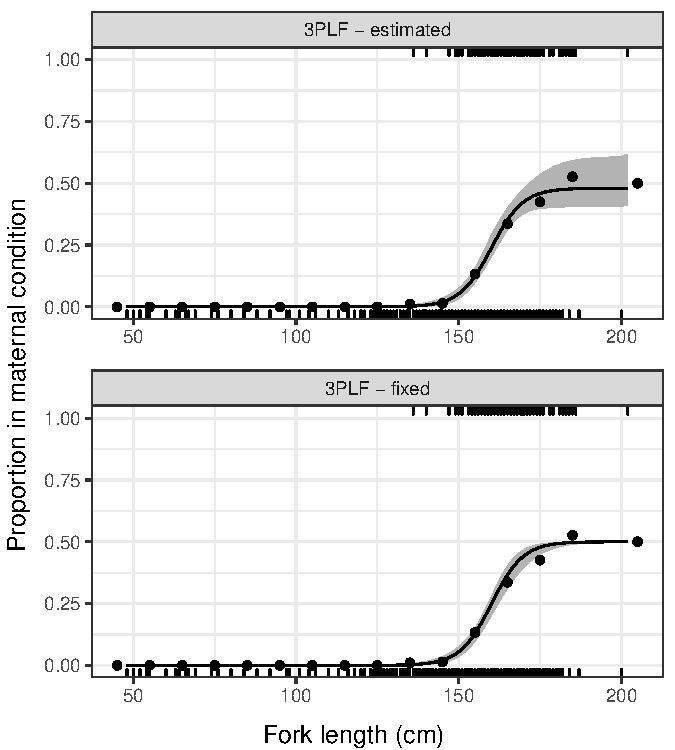
\includegraphics{/Users/avh/Library/CloudStorage/OneDrive-DepartmentofPrimaryIndustriesAndRegionalDevelopment/manuscripts/maternity-function/reports/figs_files/figure-latex/unnamed-chunk-7-1.pdf}

Figure 7. Comparison of 3PLF-estimated and 3PLF-fixed methods used to
estimate maternal parameters for sandbar shark, \emph{C. plumbeus}, in
the Gulf of Mexico and Western North Atlantic. Solid line is the
expected proportion in maternal condition at length, \(\Psi'(L)\). The
grey shaded region denotes 95\% confidence intervals based on bootstrap
resampling. Black points show proportion in maternal condition in 10cm
length intervals. Marginal rug plots denote raw data that models were
fit to. \(P_{Max}\) was fixed at 0.5 in the lower panel.

\end{document}
